% Chapter Template

\chapter{Introduction} % Main chapter title
\label{Chapter1} % for referencing this chapter elsewhere, use \cref{Chapter1}
In the recent past decades, the cancer incidence has steadily increased, affecting more than X millions of people. As shown in Figure \ref{fig:asryears}A, the incidence rate has been ever on the rise. Nonetheless, the curve of the mortality rate is dropping since the early 1990s, suggesting more effective treatments have been developed and improved over the last 20 years. Nowadays, several methods are employed to heal this disease: surgery, radiotherapy, chemotherapy, hormone therapy, targeted therapy, immunotherapy and cell-based approaches, and nuclear medicine. To achieve an effective removal of this disease, a combination of these techniques is typically applied to treat the patient. However, 

Figure XB shows both the incidence and mortality rates per 100 000 cases with respect to the body organ affected. 

Tailored treatments is currently the next step to advance further in curing cancer. The cancer relapse still represent the major cause of death. 

\begin{figure}[h!]
	\centering
	
\includegraphics[width=1.0\linewidth]{../Figures/introduction/ASR_years}
	\caption{Cancer age-standardized rate (ASR) of European Countries since the beginning of the second half of the 20th century. Data retrieved from GLOBOCAN 2022 (ref).}
	\label{fig:asryears}
\end{figure}


\begin{figure}[h!]
	\centering
	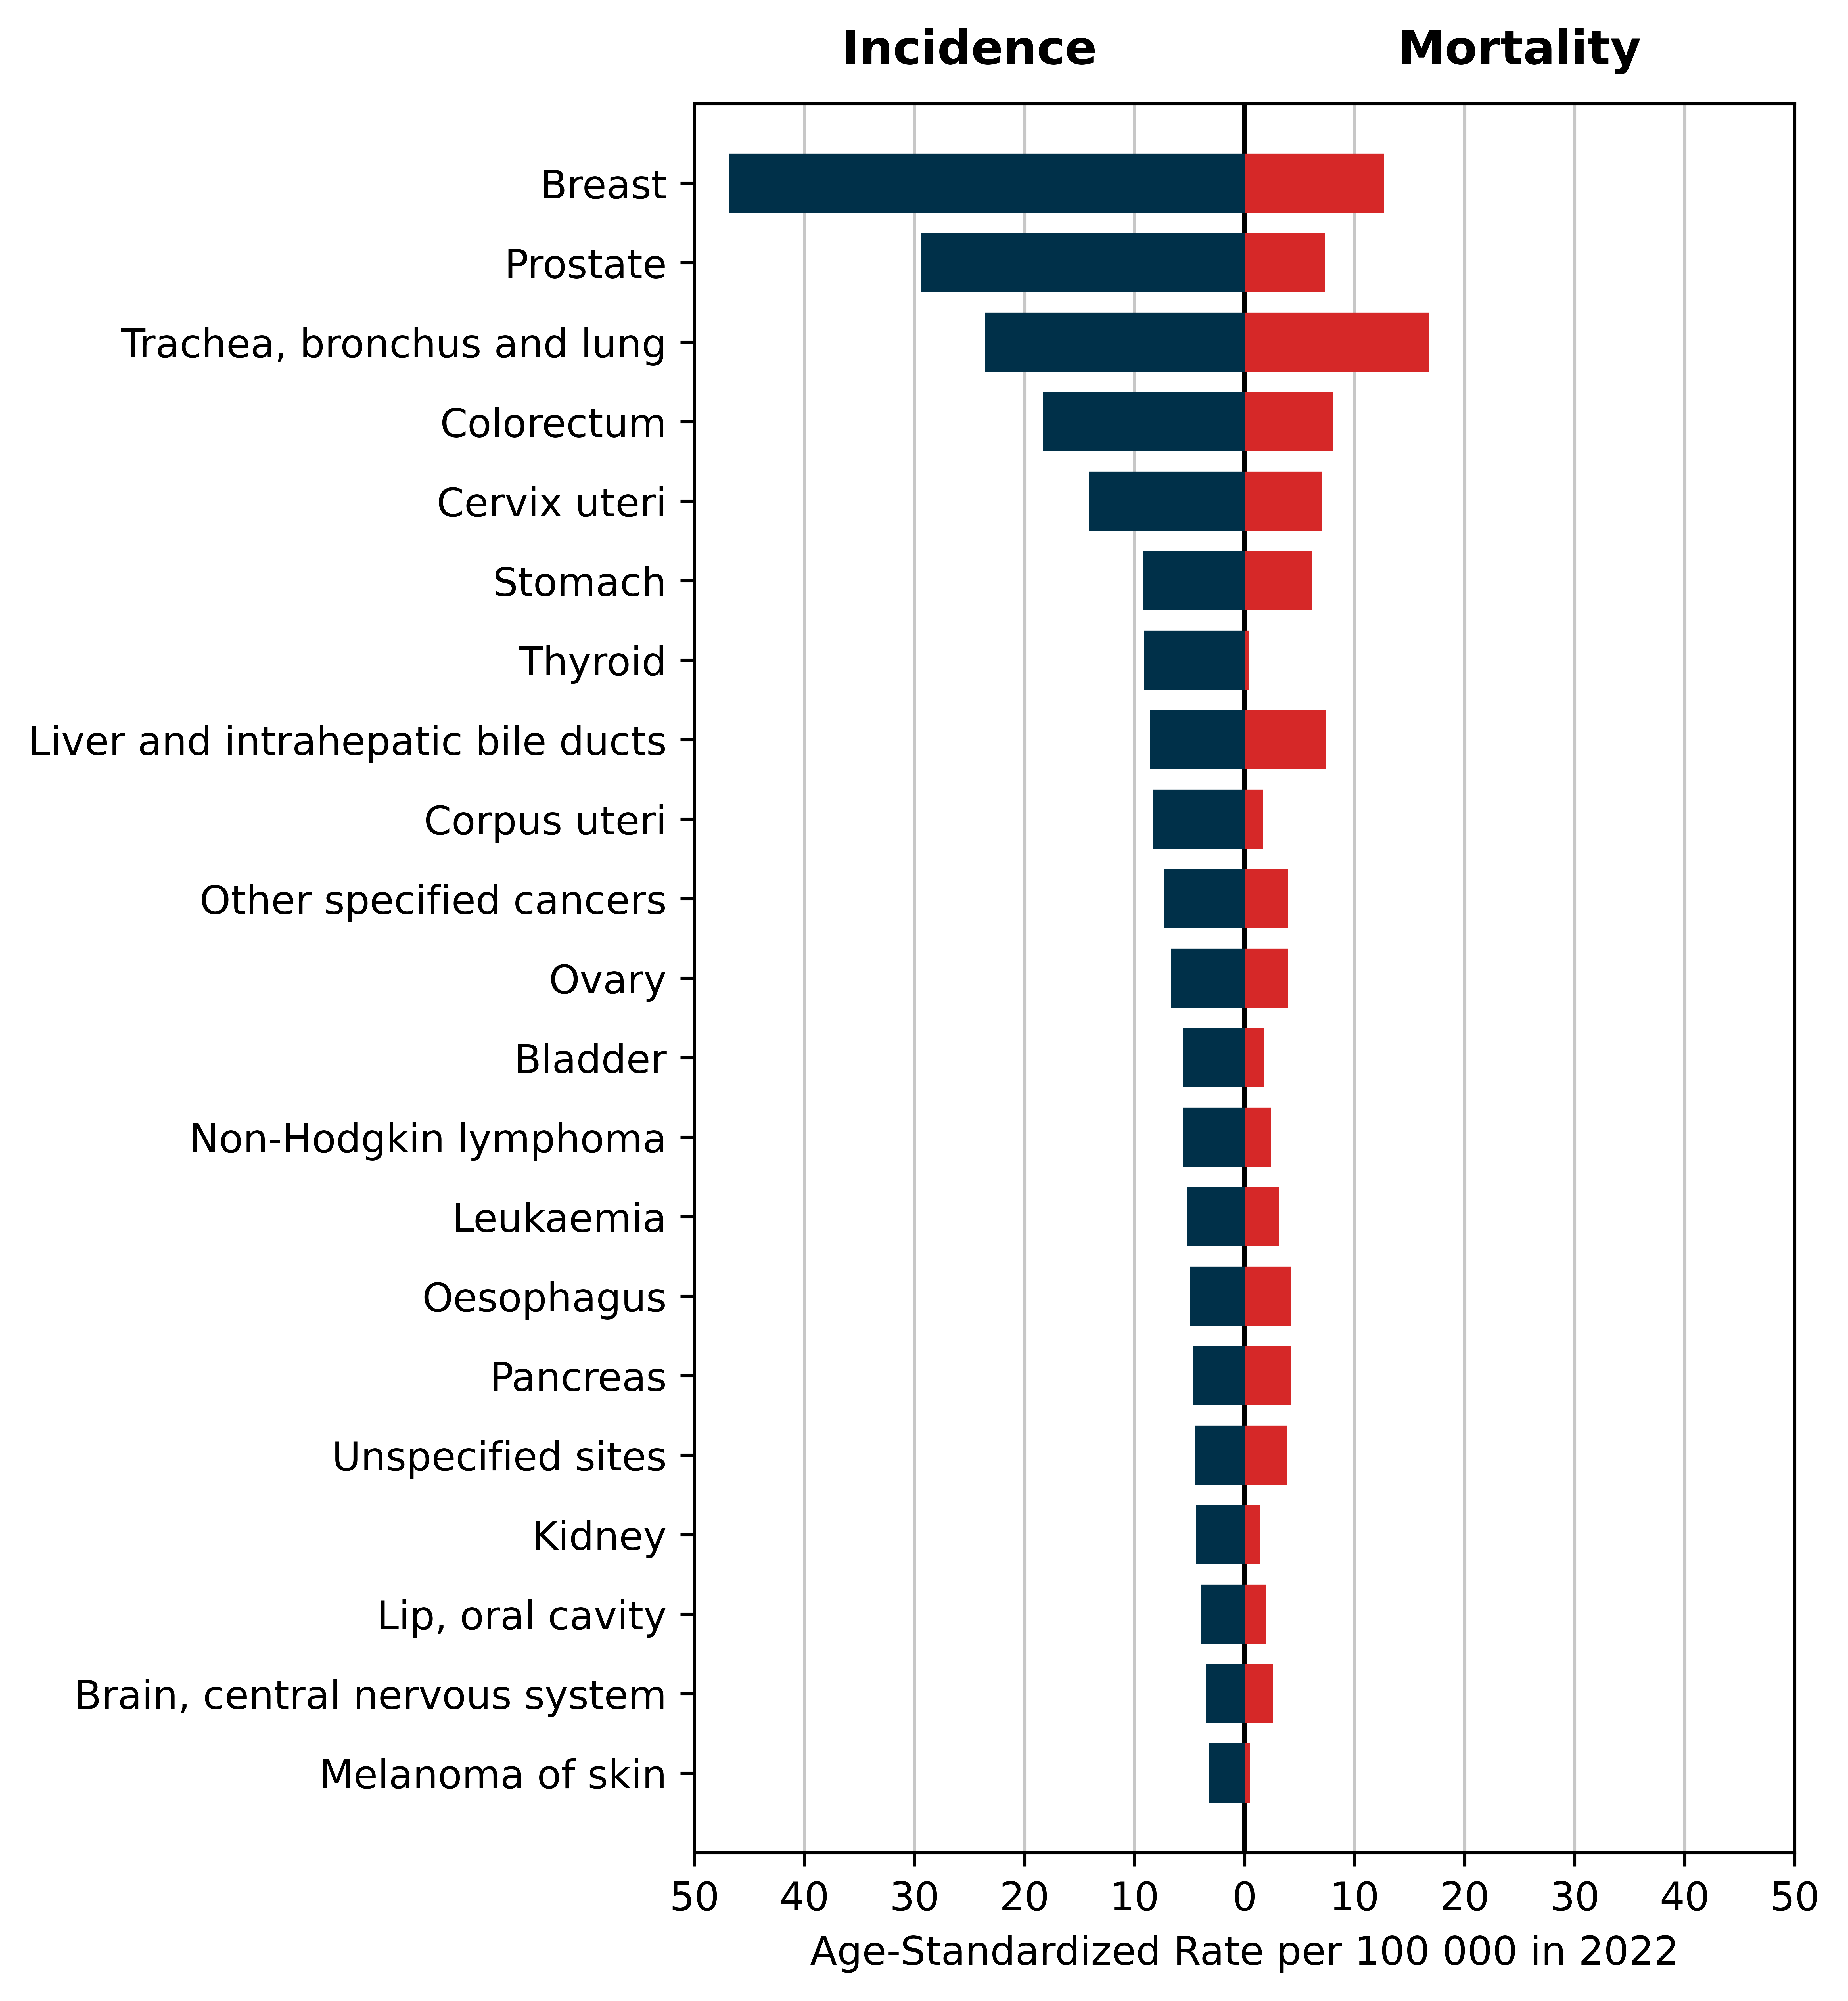
\includegraphics[width=0.7\linewidth]{../Figures/introduction/ASR_cancer}
	\caption{Incidence and mortality cancer age-standardized rate (ASR) worldwide grouped according to the organs affected. Data retrieved from GLOBOCAN 2022 (ref).}
	\label{fig:asrcancer}
\end{figure}


\section{Nuclear Medicine}
Intro nuclear medicine

\subsection{Diagnostic nuclear medicine}

\subsection{Therapeutic nuclear medicine}

\subsection{Theragnostics}

\section{Radiolanthanides in nuclear medicine}

\section{Production of medical radionuclides}

\subsection{Nuclear reactions}

\subsection{Radionuclide production workflow}

\subsection{Cross-section measurements}

\subsection{Liquid column chromatography}

\textbf{Van Deemter equation} for calculation of \acrfull{hetp} relating diffusion, mass transfer, and channeling in packed columns.

\subsubsection{Extraction chromatography}

\subsubsection{Ion exchange chromatography}

\section{Irradiation facilities}

The production of medical radionuclides is accomplished through the irradiation of target materials using several projectiles based on the final product. The neutron-rich radionuclides are typically produced using neutron fluxes available in nuclear reactors, while the neutron-deficient ones are obtained using charged particles, such as protons, deuterons, and alpha particles, typically accelerated by cyclotrons. In this work, both protons and neutrons were employed to trigger several nuclear reactions. The different irradiation facilities and their capabilities are described in details in the following subsections.

\subsection{Proton irradiation}

\subsubsection{High-intensity proton accelerator (HIPA)}
At \acrshort{psi}, a high-intensity cyclotron accelerates protons for multiple research applications. The facility is primarily utilized to generate secondary particles, such as neutrons, pions, and muons, for research in condensed matter physics, materials science, and particle physics \ref{Grillenberger2021}. This accelerator was initially named as "Meson Factory" for its initial main application of meson production. However, since its proposal occurred in the 1960s, it underwent continuous upgrades and modifications, becoming one of the most prominent accelerator facility in the world \ref{Willax1963,Grillenberger2021}. The overall accelerator is composed of a three-stage accelerator chain:
\begin{enumerate}
	\item A Cockroft-Walton DC linear accelerator, acting as a pre-accelerator generating a 870 keV proton beam;
	\item Injector II cyclotron, an isochronous separated-sector cyclotron increasing the beam energy from 870 keV to 72 MeV in less than 100 turns;
	\item Ring cyclotron, the final stage consisting of a massive isochronous machine with eight separate magnets and four main accelerating cavities. This stage accelerated the beam to its final energy of 590 MeV.
\end{enumerate}

\subsubsection{IP2 target station}

\subsubsection{Bern medical cyclotron}

\subsection{Neutron irradiation}

\subsubsection{Research reactor of the Institut Laue-Langevin}

\subsubsection{Swiss Neutron Spallation Source (SINQ)}